\chapter{Scoping and Mindset}\label{ch:ScopingMindset}
		No matter how good one gets at the technical aspects of hacking, they will never be good at it if they do not understand how to think about their target and attack.
		One must understand the difference between attempting to beat down a stone door with a battering ram and simply finding the open door behind a tree.\index{Armitage}
		In a world where the tools to run an attack are easy and often have a GUI with a big red ``hack the planet'' button,
		such as Armitage's ``hail Mary'' feature, we often forget to work out what our target is.
		This section will have you step back, away from the keyboard and look at what is happening.
		We will start with lock picking, as it is \emph{the} past time of hackers.
		Then, we will move to researching the system that you are targeting.
		However, this latter section will also require you to understand the information gathering tools explained in chapter \ref{ch:NetworkPenetration}.
	\section{Lock Picking}
	\index{Lock Picking}
		Before starting this section, you will need to either purchase or borrow a pick set and a clear or open cut lock.
		A simple hook pick and tension wrench will suffice and if you cannot find a clear lock, a cheap padlock will be easy enough to practice on.
		In this section, we will focus on the pin tumbler lock, which is the most common lock type used in cheap locking mechanisms, and the easiest to learn to pick.
		An example of this type of lock can be seen in figure \ref{fig:PinTumblerLock}.\footnote{\url{https://commons.wikimedia.org/wiki/File:Pin\_and\_tumbler\_lock\_picking.PNG}}
		Furthermore, the ideas used in this section will be added to in later chapters, notably in chapter \ref{ch:WirelessAttacks} where we will clone NFC access cards.
		\begin{figure}[htb]
			\centering
			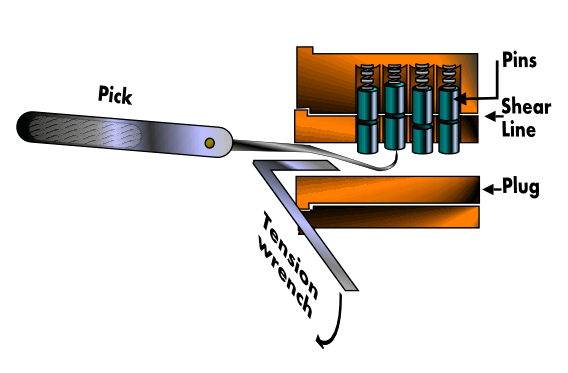
\includegraphics[scale=0.6]{./PinTumblerLock.png}
			\caption{Example of Picking a Pin and Tumbler Lock}
			\label{fig:PinTumblerLock}
		\end{figure}
		\subsection{How the Pin and Tumbler Lock Works}
			As can be seen in figure \ref{fig:PinTumblerLock}, this type of lock uses a number of sprint loaded pins which stop the plug of the lock moving within the housing.
			Within this plug is a long, thin slot for the key (or our picks) with small ledges in the sides to both stop pins from falling and hinder those attempting to pick the lock.
			A series of holes are drilled through the top of the housing and into the plug.
			These holes are where the spring loaded pins enter, with the lower pin fully entering the plug and the upper pin being split across the sheer point.
			It is this action which both allows the lock to remain closed when the key is not inserted and allows us to pick the lock.
			When a torque is placed on the plug, some of these pins will begin to bind with the sheer point.
			Using this, we can begin to pick the lock.

		\subsection{Pin by Pin Picking}
		\index{Lock Picking by Pin}
			The first step when attempting to pick a lock is to place the tension wrench into the bottom of the lock and apply a slight pressure.
			This pressure is designed to cause the top pins to catch on the sheer point of the plug, allowing some of the pins to bind.
			Once this has occurred, a pick should be used to test each of the pins, determining how many there are and which ones have become bound to the sheer point.

			The idea here is to place a small amount of pressure on the pins which bind to the sheer point in order of their binding.
			This should leave the upper pin lodged above the plug, with the lower pin dropped into the key way.
			Continue with this until either you have bound all pins and the lock is open, or you cannot determine whether pins have set or not.
			If the latter, reset the pins by releasing pressure on the tension wrench.
		\subsection{Raking}
		\index{Raking}
			If on the other hand, you are the kind of person with little patience and a strong desire to get in, you can attempt raking.
			In this process, you set the lock up in the same manner, but rather than attempting to find and set binding pins, you simply saw along the line.
			When attempting this, no more than two pins are likely to set on each pass, with passes that set no pins being common.
			Thus, you should repeatedly attempt rake until either the lock opens or you feel that you are getting nowhere.
			During this process, you may also want to slightly adjust the amount of torque placed on the plug, however, be wary not to place too much torque on it.

	\section{Problem Solving}
		Problem solving is a skill developed over time.
		However, there are numerous methods which can be followed to make it more efficient and structured.
		The following section discusses the phases of the cyber security attack life cycle, breaking them down as a problem solving methodology\cite{APTMin,AttackLifeCycleAPTOverview}.
		This cycle is shown in figure \ref{fig:CyberAttackLifeCycle}.
		\begin{figure}
			\centering
			\begin{adjustbox}{max width=1\textwidth}
			\begin{tikzpicture}[>=stealth',node distance=7cm,semithick,auto]
				\node[state]	(IR)	[text width=4cm,align=center]					{Initial Reconnaissance};
				\node[state]	(E)		[right of=IR,text width=4cm,align=center]		{Exploitation};
				\node[state]	(MA)	[right of=E,text width=4cm,align=center]		{Maintaining Access};
				\node[state]	(AP)	[below of=MA,text width=4cm,align=center]		{Appropriating Privileges};
				\node[state]	(IntR)	[left of=AP,text width=4cm,align=center]		{Internal Reconnaissance};
				\node[state]	(PI)	[left of=IntR,text width=4cm,align=center]		{Pivoting to Internal Systems};
				\node[state]	(EX)	[above left of=PI,text width=4cm,align=center]	{Exfiltration};

				\draw[->] (IR)		-> (E);
				\draw[->] (E)		-> (MA);
				\draw[->] (MA)		-> (AP);
				\draw[->] (AP)		-> (IntR);
				\draw[->] (IntR)	-> (PI);
				\draw[->] (PI)		-> (EX);
				\draw[->] (EX)		-> (IR);
				% \path[->] (IR) 	edge (E)
				% 				edge (MA)
				% 				edge (AP)
				% 				edge (IntR)
				% 				edge (PI)
				% 				edge (EX)
				% 				edge (IR);
			\end{tikzpicture}
			\end{adjustbox}
			% 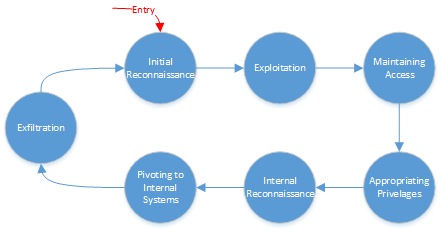
\includegraphics[scale=0.8]{./AttackLifeCycle.png}
			\caption{The Cyber Security Attack Life Cycle}
			\label{fig:CyberAttackLifeCycle}
		\end{figure}
		\index{Cyber Security Attack Cycle}
		\subsection{Initial Reconnaissance}
			Before starting any attack, you need to have a point of entry into the system.
			This may be a small piece of knowledge, or data about the system, or it may be a glaring hole in the wall in front of you.
			However, it is also the slowest and most fundamental part of the process.
			To be useful, it must go through multiple phases:
			\begin{enumerate}
				\item \textbf{Open Discovery:} Using open source intelligence to discover both the operations and workings of the target.
				\item \textbf{Activity Analysis:} Using the information discovered in step 1, determine what activities are being conducted to allow the events which you are looking into.
					If this is an organisation, work out their procedures.
					If this is a task or other problem, work out it's intricacies.
				\item \textbf{Host Enumeration:} This lists every option for moving forward with exploitation.
					It does not attempt to evaluate them, but rather listing them for further study.
				\item \textbf{Passive Scanning:} Listening to traffic which is accessible and passing from the target.
				\item \textbf{Active Scanning:} Making requests of the hosts found in stage 2 in order to discover their workings and vulnerabilities.
				\item \textbf{Host Evaluation:} Using the data gathered above, deciding which host to attack first.
				\item \textbf{Attack Preparation:} Final preparation of yourself and your environment for the attack
			\end{enumerate}

			By following this process, or a derivative of it, you should understand exactly what you will be targeting in the next phase.
			You should have exactly one target that you know exactly how you will exploit it.
			However, you should also have numerous other targets, such that if the first were to fail, you would be able to recover using one of these.
			The information that is gathered here should be retained permanently, as it is an exceptional resource in the later phases.

		\subsection{Exploitation}
			You have already decided on how you will enter the system, you must now craft the exploit which will make it happen.
			This involves generating the payload that you will send in a specific manner.
			You must intimately know your target so that anything you send will be successful.
			Furthermore, you should build the exploit in such a way that you will receive confirmation and a request for more information, should it be successful.
			This allows you not only to know whether it worked, but also to keep inserting new code or ideas into your target.

			This phase is the hardest, relying absolutely on the previous phase.
			You are stepping over the boundary between being inside the system and being outside.
			This is where most defences lay, and where most of the attacks that get caught do so.
			Thus, it should be a careful, meticulous process, rather than a rushed smash and grab.
		\subsection{Maintaining Access}
			Your foot is in the door, you must now firmly remove the lock and ensure it doesn't get replaced.
			This phase gives you the ability to return whenever you need, making it the only way to completely achieve your mission.
			There are numerous ways to do this, each with their own issues and benefits:
			\begin{description}
				\item[Blending in with the crowd] Become just another user, or another admin.
					This method requires that you create an account for yourself, making all future access seem legitimate.
					It has the benefit of giving you authorised access that is hard to find in large systems or organisations.
					However, you lose the benefit of your original attack tools, meaning that you have to attack again to be able to use your pivoting infrastructure without building it manually.
				\item[Listeners] Ensure that someone or something is looking out for you, waiting for you to call again.
					This works by inserting code that constantly runs waiting for you to connect.
					It has the benefit of giving you access to your attack tools (if created by them)
					but is vastly easier to find as it leaves an open port and code stored on disk.
				\item[Beacons] Why call them when they can call you?
					This will leave a program on the system which will attempt to initiate connections back to you at a given time.
					It is generally as beneficial as a listener, with the exception that it is more likely to bypass a firewall,
					making it far more reliable once set up.
					However, it does also leave an address to use to contact you on their device, making it easier to detect what you are doing.
			\end{description}
			These latter two do not always come with security by default.
			You may be the attacker, but you are not the only one.
			If at all possible, you should ensure that you are the only one who can walk through the doors that you have opened.
			That way, they will always be open to you alone, and will not be stolen and blocked off by someone else.

			You should always ensure that you have at least one, preferably two of these in use.
			Even if you don't think you will ever return to the exploited machine, there is no reason to close an open door.
		\subsection{Appropriating Privileges}
			You're in the system, you can walk in or out whenever you want; at this point, the security guard probably thinks he knows you by first name.
			However, you're far from winning yet.
			Before you can move any further, you need to find a way to gain more access.
			While you may currently be able to walk in the front door, the elevator will only take you to floors 1 through 5, and our goal is in the basement.

			This phase requires you to start again on a smaller scale.
			You have access into a small portion of your final goal, you now have to find an exploit which will give you the whole machine, letting you start on taking the whole organisation or network.

			Starting again from reconnaissance, you should look at all the programs running on the compromised system.
			These will likely give you a way to improve your credentials on the machine, allowing you to move on to the next phase of the attack.

		\subsection{Internal Reconnaissance}
			You truly have your foot in the door now.
			More to the point, you can walk freely around the building nattering with security.
			However, your target is in the next system along, or the next building.
			This phase is about looking around the local network and finding where that target is.

			Using the access you have gained, you should be able to install the tools required to use this machine as a view port to the rest of the network.
			Conduct the activities discussed in Initial Reconnaissance above, with less of a focus on open source and more on scanning and sniffing.

			This phase should not only tell you where your next target is, but also how you will get into it.
			It is either your second last barrier to success, or an iteration towards it.
		\subsection{Pivoting to Internal Systems}
			This is your final barrier to success.
			You now need to break into the target system, the one that holds the information or performs the services that you need.
			This process should be the same as the initial exploit on the network.
			You need to craft an attack which will get you in unnoticed, allowing you the time you need to find what you are looking for.
			Follow the same steps you did in exploitation above, and you will gain entry into the target system, finally giving you access to your goal.
		\subsection{Exfiltration}
			Your target is sitting right in front of you now.
			There are no guards any more, they are still watching the front door that they let you walk through months ago.
			All that you need to do is send the data you are looking for back, or alter the service that you had originally aimed for.
			However, now is not the time for burning bridges.

			Even though you have succeeded, you should take it slow at this point.
			If anyone at all is monitoring the network, they will notice the large amount of data following an odd path out of their network.
			Thus, you should use peak traffic times and low data rates to exfiltrate.
			Making sure that you prioritise what you take, you should be able to set the process in motion and wait for it to finish.

			Whether your goal was simple or complex, do not break down the access that you have gained.
			Leave it in place, because it will become useful if you need to gain access to the same network again.
			As previously stated, there is no point closing doors that you might need later.

		\subsection{Conclusion}
			If you have read through to this point and do not see how this relates to problem solving, it will come.
			While all of it may seem purely based on cyber attacks and technology, it does have a mindset that is useful to any problem.
			Before compartmentalizing this methodology as cyber security only, try it with a real world problem.
			War game through it in this way before making any choices, then decide, exploit and build a level of access.
			It may seem slow, but that is only because it is methodical, silent and vicious.

